\subsection{Visualisierung der Klassifikation durch Annotationen}
    Eine wichtige Funktion des \glspl{wccs}
    ist die Visualisierung einer Klassifikation durch Webannotationen
    auf der klassifizierten Webseite.
    Aus diesem Grund folgt eine Übersicht der Annotationen
    des Studienportals \gls{babw},
    welches stellvertretend auch für die restlichen klassifizierten Portale steht.
    Abbildung \ref{image:findingTeachersAnnotationsOverview}
    zeigt einen Ausschnitt der annotierten
    Seite\footnote{Die Darstellungsfehler oben rechts im Kopfbereich
    sowie am Anfang der Brotkrümelnavigation unter dem Portal
    sind dem in Kapitel \ref{section:findingsMethod} beschriebenen
    Annotation Viewer geschuldet.
    Durch die Zwischenschaltung dieser Komponente
    führt der Browser Cross-Origin-Requests durch,
    um die genutzte Bibliothek für Symbole zu beziehen.
    Diese Aufrufe werden allerdings unterbunden,
    weshalb die Symbole nicht korrekt dargestellt werden.
    Bei einer direkten Einbindung des Plugins wäre dies nicht der Fall.
    Der fünfte Link im Kopfbereich wurde richtig klassifiziert.}.

    \begin{figure}[htb]
        \centering
        
\includegraphics[width=\textwidth]{../resources/findings/case-study-1/babw/annotations/overview.png}
        \caption{Annotierte Seite über Lehrenden und Betreuenden im \acrshort{babw}}
        \label{image:findingTeachersAnnotationsOverview}
    \end{figure}

    Bis auf wenige Ausnahmen, die in unter anderem in
    Kapitel \ref{section:findingsTeachersAbnormalitiesBabw} besprochen werden,
    wurden alle klassifizierten Elemente korrekt hervorgehoben.
    Eine detaillierte Ansicht eine beispielhaften Annotation zeigt
    Abbildung \ref{image:findingTeachersSubjectAreaAnnotations}.

    \begin{figure}[htb]
        \centering
        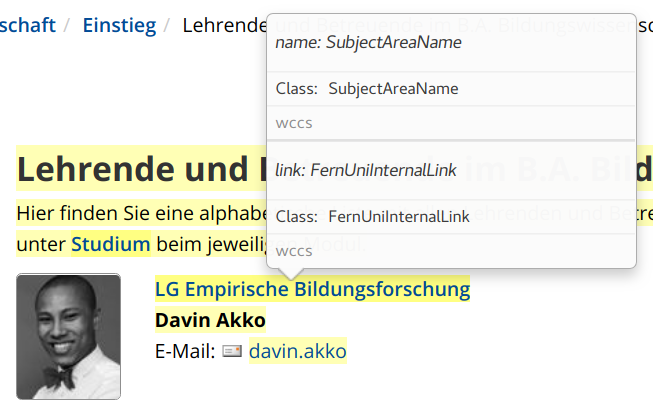
\includegraphics[scale=\screenshotScaleFactor]{../resources/findings/case-study-1/babw/annotations/double-lg-annotation.png}
        \caption{Annotationen eines Lehrgebietes}
        \label{image:findingTeachersSubjectAreaAnnotations}
    \end{figure}

    Das Lehrgebiet besitzt korrekterweise zwei Annotationen,
    da das HTML-Element sowohl den Namen als auch den Link enthält
    und deshalb doppelt klassifiziert wurde.